\documentclass{article}

\usepackage{fontspec}
\usepackage{polyglossia}
\usepackage{notomath}
\setmainfont{GFS Artemisia}
\setsansfont{Source Code Pro}
\setmonofont{Source Code Pro}
\newfontfamily\greekfont[Script=Greek]{GFS Artemisia}
\newfontfamily\greekfontsf[Script=Greek]{GFS Artemisia}
\newfontfamily\greekfonttt[Script=Greek]{Source Code Pro}

%languages
\setdefaultlanguage{greek}
\setotherlanguages{english}


%typing
\usepackage{hyphenat}
\usepackage{float}
\usepackage{color, colortbl}
\usepackage{placeins}

%captions
\usepackage{caption}
\usepackage{subcaption}

%bib
% \usepackage{biblatex}
% \addbibresource{bib.bib}

%gemoetry
\usepackage[a4paper,top=1.2cm,bottom=1.2cm,left=1.2cm,right=1.2cm,marginparwidth=1.5cm]{geometry}

%images
\usepackage{graphicx}
\usepackage{tikz}

%ref
\usepackage[colorlinks=true, allcolors=blue]{hyperref}


\usepackage[export]{adjustbox}

%label
\usepackage{enumitem}
\renewcommand{\labelenumii}{\arabic{enumi}.\arabic{enumii}}
\renewcommand{\labelenumiii}{\arabic{enumi}.\arabic{enumii}.\arabic{enumiii}}
\renewcommand{\labelenumiv}{\arabic{enumi}.\arabic{enumii}.\arabic{enumiii}.\arabic{enumiv}}

%columnnew
\newcolumntype{g}{>{\columncolor{gray}}l}

%colors
\usepackage[dvipsnames]{xcolor}
\definecolor{gray}{gray}{0.9}
\definecolor{blue}{RGB}{82, 138, 174}
\definecolor{green}{RGB}{140, 219, 169}
\definecolor{yellow}{RGB}{253, 221, 92}

% \usepackage{titling}
% \setlength{\droptitle}{-20em}             %allagh glwssas
\hypersetup{
    colorlinks = true,
    linkcolor=black}


\usepackage{autobreak}


%Customize tables
\renewcommand{\arraystretch}{1.2}
% \rowcolors{2}{gray}{white}



\captionsetup[table]{
    format=plain,
    labelfont={small,it,bf}, % Small, italic, and bold label
    textfont={small,it}, % Italic text
    labelsep=colon % Colon separator
}



% Customize the figure caption
\captionsetup[figure]{
    format=plain,
    labelfont={small,it,bf}, % Small, italic, and bold label
    textfont={small,it}, % Italic text
    labelsep=colon % Colon separator
}

\makeatletter
\renewcommand*{\p@table}{\textit{Πίν. }}
\renewcommand*{\p@figure}{\textit{Σχ. }}
\renewcommand*{\p@equation}{\textit{Εξ. }}
\makeatother


\begin{document}

%TITLE
\newcommand{\uni}{ΑΡΙΣΤΟΤΕΛΕΙΟ ΠΑΝΕΠΙΣΤΗΜΙΟ ΘΕΣΣΑΛΟΝΙΚΗΣ}
\newcommand{\faculty}{ΠΟΛΥΤΕΧΝΙΚΗ ΣΧΟΛΗ}
\newcommand{\tmhma}{ΤΜΗΜΑ ΜΗΧΑΝΟΛΟΓΩΝ ΜΗΧΑΝΙΚΩΝ}


\newcommand{\titlos}{Δυναμικά φαινόμενα}
\newcommand{\ypotitlos}{Bonus Εργασία - Ειδικά Κεφάλαια Πεπερασμένων Στοιχείων}


\newcommand{\onomaauthor}{ΒΑΣΙΛΕΙΟΣ ΠΑΠΑΜΙΧΑΗΛ}


\newcommand{\advisor}{Γάκιας Χρήστος}
\newcommand{\mailauthor}{\href{mailto:vasilepi@meng.auth.gr}{vasilepi@meng.auth.gr}}
\newcommand{\aem}{6920}
\newcommand{\hmeromhnia}{\today}



\begin{titlepage}
    \begin{center}
    \raisebox{20mm}{
    \begin{tikzpicture}
        \draw (0,0) -- (6,0);
    \end{tikzpicture}}
\includegraphics[width=4cm]{media/autheng.jpg}\raisebox{20mm}{\begin{tikzpicture}
        \draw (0,0) -- (6,0);
    \end{tikzpicture}}
     \end{center}
    
    \begin{center}
        \large
        \uni\\
        \normalsize
        \faculty\\
        \vspace{1em}
        \tmhma
    \end{center}

    \vspace{2cm}
    \begin{center}
        \Large
        \textbf{\titlos}\\
        \vspace{1em}
        \large
        \textit{\ypotitlos}
    \end{center}
    \begin{center}
        \begin{tikzpicture}
        \draw (0,0) -- (4,0);
    \end{tikzpicture}\\
    \vspace{7em}
    \Large
    \textcolor{BrickRed}{\textbf{\onomaauthor}}\\
    \vspace{3em}
    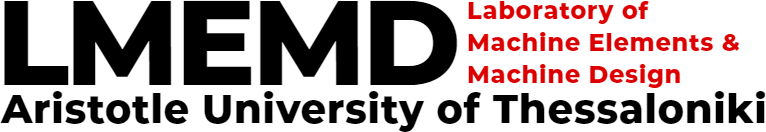
\includegraphics[width=0.3\textwidth]{media/newlogov3-cropped-content.png}
    \end{center}

    \vspace{7em}
    \hspace{4ex}
    \begin{minipage}[t]{0.45\textwidth} 
        \raggedright
        \textbf{Υπεύθυνος}: \advisor\\
        \textbf{Email}: \mailauthor\\
        \textbf{ΑΕΜ}: \aem
    \end{minipage}\\

    \vspace{4cm}
    \begin{center}
        \textit{\hmeromhnia}\\
        \begin{tikzpicture}
            \draw (0,0) -- (15,0);
        \end{tikzpicture}
    \end{center}
    
    
\end{titlepage}

\tableofcontents


\section{Εισαγωγή}
\subsection{Παρουσίαση προβλήματος}
Σκοπός της παρόν εργασίας είναι η επίλυση προβλημάτων επαφών και η εξακρίβωση των αποτελεσμάτων μέσω της θεωρίας επαφών κατά Hertz και της μεθόδου της ποινής. Η εργασία χωρίζεται σε δύο μέρη. 
\par Στο πρώτο μέρος ζητείται η δημιουργία κώδικα που επιλύει απλό πρόβλημα επαφής μεταξύ δύο ράβδων. Τα άκρα των δύο ράβδων είναι πακτωμένα. Οι ράβδοι έχουν αρχικά απόσταση μεταξύ τους. Έπειτα, το ελεύθερο άκρο της μίας ράβδου μετατοπίζεται με τη βοήθεια δύναμης προς την άλλη ράβδο. Μόλις οι δύο ράβδοι βρεθούν σε επαφή επιλύεται το πρόβλημα με τη μέθοδο της ποινής. Ζητούνται τα διαγράμματα δύναμης-μετατόπισης, τα μητρώα στιβαρότητας, τις αναπτυσσόμενες τάσεις και τη δύναμη επαφής.

\begin{figure}[H]
    \centering
    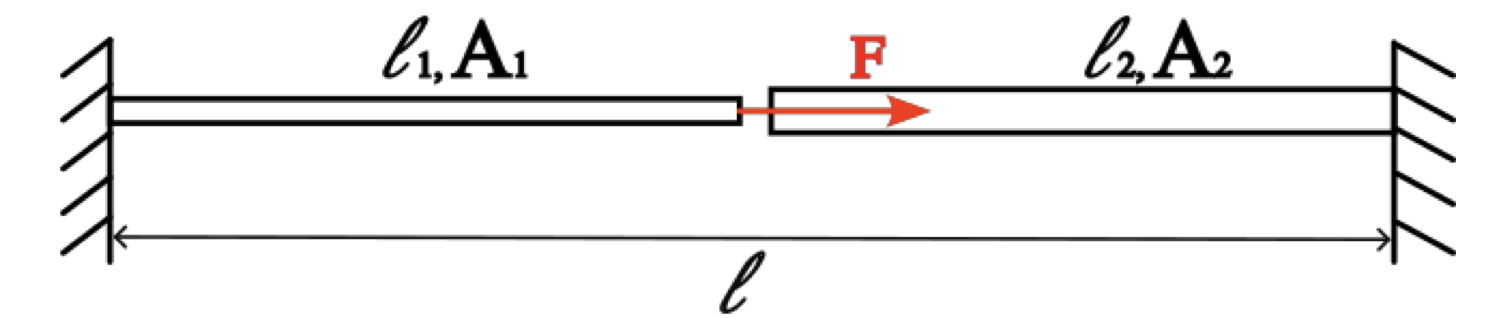
\includegraphics[width=0.6\linewidth]{media/merosA.png}
    \caption{Πρόβλημα πρώτου μέρους.}
    \label{fig:merosA}
\end{figure}

\par Στο δεύτερο μέρος διερευνάται η γραμμική και η σημειακή επαφή μέσω της θεωρίας του Hertz. Ζητείται η δημιουργία δύο μοντέλων για την επίλυση των δύο προβλημάτων. Για τη γραμμική επαφή, δημιουργείται μοντέλο ΠΣ δύο κυλίνδρων σε επαφή. Η δύναμη ασκείται στον έναν κύλινδρο και αναπτύσσονται έτσι οι τάσεις επαφών. Για τη σημειακή επαφή μελετάται η περίπτωση επαφής σφαίρας με επίπεδο. Τα προβλήματα αυτά θα επιλυθούν τόσο με αδρό πλέγμα όσο και με πυκνό. Οι επιλύσεις θα συγκριθούν με τα θεωρητικά αποτελέσματα από τη θεωρία του Hertz. Τα ζητούμενα είναι η αναπτυσσόμενη πίεση και το πλάτος επαφής, οι αναπτυσσόμενες κύριες τάσεις, η σχέση δύναμης-μετατόπισης.
\begin{figure}[H]
    \centering
    \begin{subfigure}{0.49\linewidth}
        \centering
        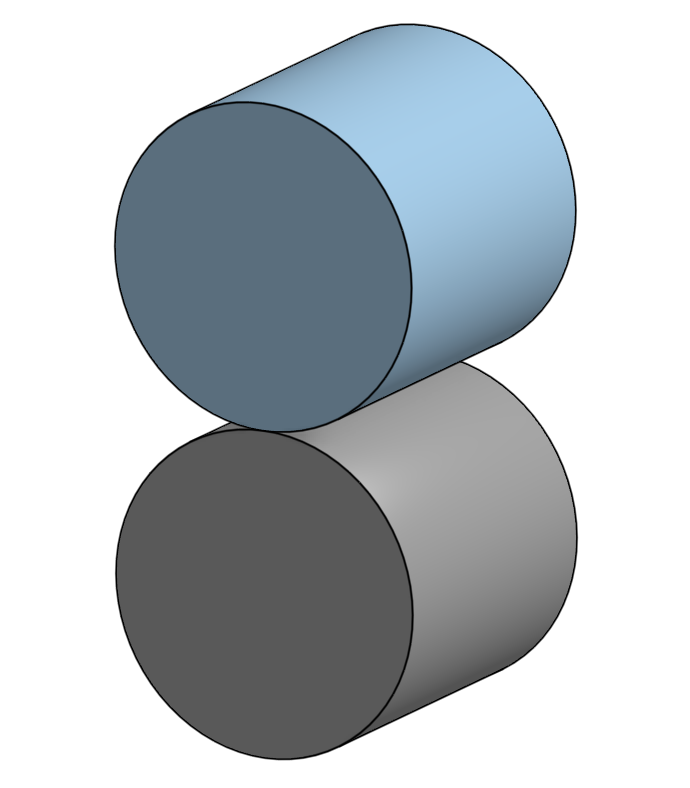
\includegraphics[width=0.6\linewidth]{media/kyl.png}
        \caption{Πρόβλημα γραμμικής επαφής.}
    \end{subfigure}
    \hfill
    \begin{subfigure}{0.49\linewidth}
        \centering
        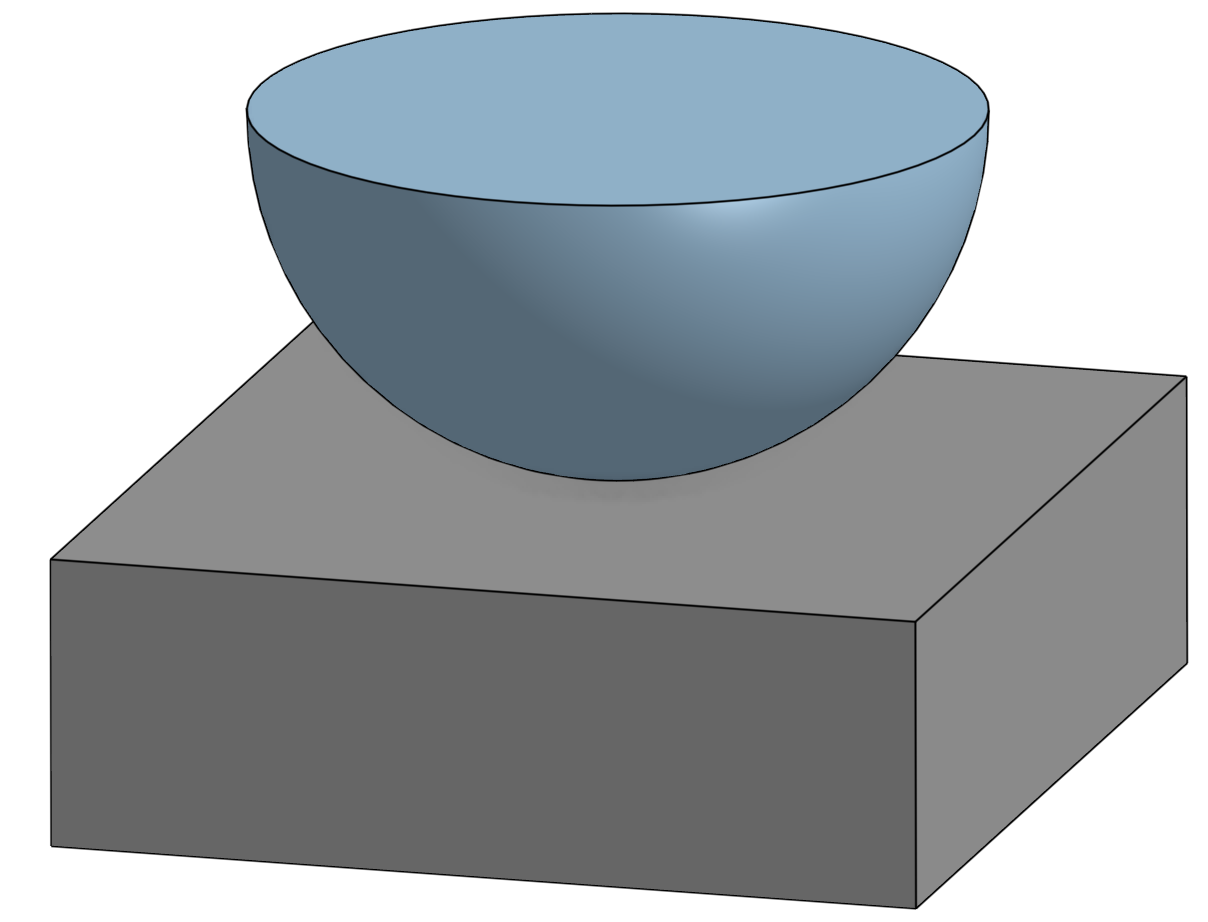
\includegraphics[width=0.6\linewidth]{media/sfaira.png}
        \caption{Πρόβλημα σημειακής επαφής.}
    \end{subfigure}
    \caption{Προβλήματα δεύτερου μέρους.}
    \label{fig:merosB}
\end{figure}



\subsection{Συνοπτική θεωρία}
\subsubsection{Μέθοδος ποινής}

\subsubsection{Θεωρία Hertz}

\begin{align}
    &F_1-F_2-u(k_1+k_2)=0\\
    &F_1+F_2=0
\end{align}

\begin{equation}
    \vec{F} = \begin{bmatrix}
        F_1\\
        F_2
    \end{bmatrix},\; \vec{u}=\begin{bmatrix}
        u\\
        0
    \end{bmatrix},\; K_i = \begin{bmatrix}
        k_1+k_2 & 0\\
        0 & 0\\
    \end{bmatrix},\; A = 
    \begin{bmatrix}
        1 & -1\\
        1 & 1
    \end{bmatrix}
\end{equation}
\begin{equation}
    A\cdot \vec{F} - K_i \cdot \vec{u} = \vec{0}
\end{equation}

\begin{equation}
    \vec{F} - A^{-1}\cdot K_i \cdot \vec{u} = \vec{0} 
\end{equation}

\begin{equation}
    K = A^{-1}\cdot K_i
\end{equation}

\begin{equation}
    \Pi = \frac{1}{2}K\vec{u} \vec{u}^T - \vec{F} \vec{u}^T
\end{equation}

\begin{equation}
    g = \begin{bmatrix}
        H-(l+u)\\
        H-l
    \end{bmatrix},\; \epsilon=\begin{bmatrix}
        a & b \\
        c & d
    \end{bmatrix}, a,b,c,d >> k_1+k_2
\end{equation}

\begin{equation}
    \Pi_p = \frac{1}{2}K\vec{u} \vec{u}^T - \vec{F} \vec{u}^T - \frac{1}{2}\epsilon \vec{g} \vec{g}^T = \begin{bmatrix}
        x & y\\
        z & w
    \end{bmatrix}_{2\times 2}
\end{equation}

\begin{align}
    \frac{\partial x}{\partial u} &= 0\\
    \frac{\partial y}{\partial u} &= 0\\
    \frac{\partial z}{\partial u} &= 0\\
    \frac{\partial w}{\partial u} &= 0
\end{align}

\begin{equation}
    \vec{N} = -\epsilon \vec{g}
\end{equation}


\end{document}